\documentclass[12pt,a4paper]{report}

\title{Sistema de extracción automática de información de documentos}
\author{Daniel González Cerviño}
\date{\today}

% Configure languaje and codification
\usepackage[utf8]{inputenc}
\usepackage[spanish]{babel}
\selectlanguage{spanish}

% Image manipulation
\usepackage{graphicx}
\usepackage{tikz}
% Allow title personalization
\usepackage{titlesec}
% Allow use TrueType and Open Type fonts
\usepackage{fontspec}
\usepackage{lmodern}
% Allow use font colors
\usepackage{xcolor}
% Allow tables with 100% width
\usepackage{tabularx}
% Allow reference last page of document
\usepackage{lastpage}
% Allow advanded tools for headers and footers.
\usepackage{fancyhdr}

% Set margins
\usepackage[top=3.5cm,bottom=3.5cm,left=2.75cm,right=2.75cm,]{geometry}
\usepackage[T1]{fontenc}
\pagestyle{plain}

% Set headers and footers
\fancypagestyle{plain}{%
    \renewcommand{\headrulewidth}{0pt}
    \fancyhead{}
    \fancyfoot{}
    \fancyfoot[R]
    {{ Sistema de extracción automática de información de documentos | \scriptsize\thepage\ de \pageref{LastPage}}}
    \fancyhead[L]
    {\tikz[remember picture,overlay]\node[opacity=0.4] at (-3mm, 10mm){
\includegraphics[scale=0.18]{./images/header}};}
    \fancyheadoffset{0pt}
}

\pagestyle{plain}

\begin{document}

% cover
    \begin{titlepage}

    \tikz[remember picture,overlay]
    \node[opacity=1,inner sep=0pt] at (77mm, -110mm)
        {
\includegraphics{./cover/images/cover}};

    \vspace{50em}
    \fontspec{Oswald}[BoldFont={Oswald-Bold}]
    \fontsize{28}{10.4}\selectfont
    \color{white}
    \begin{flushleft}
        \textbf{Sistema de extracción de información de documentos}
    \end{flushleft}

    \restoregeometry
\end{titlepage}

%    \noindent
\Huge\textbf{Trabajo final de grado}
\normalfont\normalsize
\vspace{3em}
\begin{table}[h]
    \renewcommand{\arraystretch}{1.5}
    \begin{tabular}{p{0.35\textwidth} p{0.65\textwidth}}
        \hline\textbf{Título}             & Sistema de extracción automática de información de documentos \\
        \hline\textbf{Universidad}  & Universidad Internacional de Valencia                         \\
        \hline\textbf{Titulación}   & Grado de ingeniería informática                               \\
        \hline\textbf{Mención}      & Ingeniería del software                                       \\
        \hline\textbf{Curso}        & 2023/24                                                       \\
        \hline\textbf{Convocatoria} & Primera convocatoria, Junio                                   \\
        \hline\textbf{Autor}        & Daniel González Cerviño, 49012312 W                           \\
        \hline\textbf{Directora}    & Marlene Goncalves Da Silva, Y7592198 G                        \\
        \hline
    \end{tabular}
    \label{tab:}
\end{table}




\tableofcontents
    \addcontentsline{toc}{chapter}{\listfigurename}
    \addcontentsline{toc}{chapter}{\listtablename}
    \listoffigures
    \listoftables

% Dedication
    \newpage
\section*{Dedicatoria}

A Arancha, mi compañera incansable, cuyo apoyo ha sido fundamental en este proceso.
Gracias por asumir, con amor y sin quejas, la carga extra de nuestras responsabilidades familiares para que yo pudiera
concentrarme en este proyecto.
Tu fortaleza y dedicación son el cimiento de nuestra familia y de cada uno de mis logros.

A mis queridas hijas, Aroa y Enara, gracias por llenar cada día con vuestra alegría y vuestras ganas de vivir.
Vuestra energía y felicidad han sido la fuente de mis fuerzas y la luz en los momentos de oscuridad.
Os pido perdón por las veces que la consecución de este grado me ha apartado de vosotras, robándome momentos juntos.

Este trabajo es tan vuestro como mío.
Dedicado con todo mi amor y gratitud a las tres, por ser mi mayor inspiración y el motivo de mi esfuerzo.


% Abstract
    \providecommand{\keywords}[1]
    {
        \small
        \textbf{\textit{keywords :\hspace{0.3cm}}} #1
    }
    \providecommand{\keywords}[1]
{
    \small
    \textbf{\textit{keywords: \hspace{0.3cm}}} #1
}
\begin{abstract}
    \todo[inline]{@TODO: completar al final}
    Es una sección concisa y precisa (400 a 500 palabras) que resume los aspectos más importantes del trabajo
    realizado. Su objetivo es proporcionar una visión general rápida y clara del contenido y los resultados obtenidos,
    capaz de captar la atención e interés del lector, invitándolo a leer el trabajo completo.
    El resumen debe comenzar con una breve introducción que contextualice el tema del trabajo y exponga la problemática
    abordada. Debes mencionar de manera breve los objetivos o propósitos principales del trabajo. Brevemente, describe
    los métodos/metodología o enfoque que has utilizado para llevar a cabo el trabajo. Resume los principales resultados
    obtenidos. Indica las conclusiones o contribuciones más importantes derivadas de tu trabajo.
    Palabras clave: Al final del resumen, proporciona una lista de palabras clave que representen los conceptos
    principales y los temas abordados en tu trabajo.

    \vspace{0.5cm}
    \keywords{primero, segundo, tercero}
\end{abstract}


%% Chapters
    \chapter{Introducción}\label{ch:chapter_1}


\section{Antecedentes}

El desarrollo de este Trabajo de Fin de Grado (TFG) surge de una necesidad surgida en mi faceta profesional, donde la
tarea repetitiva de leer y extraer información de documentos representa una carga significativa para la empresa en la
que trabajo.

Este desafío no es exclusivo de mi actual empresa actual, sino que es una realidad común en una variedad de sectores
incluyendo entre otros:

\begin{itemize}
    \item Compañías de seguros
    \item Instituciones educativas
    \item Empresas del sector sanitario
    \item Empresas de gestión de recursos humanos
    \item Entidades financieras
\end{itemize}

Estas organizaciones enfrentan el reto constante de gestionar grandes volúmenes de documentación, lo cual resalta la
importancia y la necesidad universal de soluciones automatizadas que permitan extraer información de los mismos.

Durante la asignatura del Grado de Ingeniería Informática 47 Proyecto de Ingeniería del Software, tuve la oportunidad de
desarrollar una base técnica preliminar que se ha convertido en la base para la realización de este proyecto.


\section{Planteamiento del problema}

Estas tipologías de empresas que hemos visto en el apartado anterior se enfrentan a la necesidad de procesar una enorme
cantidad de documentos.

Por ejemplo una empresa que gestiona seguros de coche, deberá recibir un paquete de datos de cada nuevo cliente que
contendrá entre otros los siguientes documentos: documento de identidad del titular y los tomadores, carne de conducir
de los tomadores, ficha técnica del vehículo,permiso de circulación, recibo del impuesto de vehículo de tracción
mecánica.

La forma tradicional de obtener la información de dichos documentos consiste en que un operario reciba los datos y los
introduzca en el sistema.
Esta metodología tradicional enfrenta una problemática significativa:

\begin{itemize}
    \item \textbf{Elevado coste financiero}
    El personal dedicado a estas tareas genera un gasto que impacta directamente en el coste operativo de la
    organización
    \item \textbf{Demora en los tiempos de tramitación}
    La tramitación manual implica que los documentos no van a ser procesados en el tiempo en que son recibidos, sino
    que deberán esperar a que un operario esté disponible para ocuparse de esta tarea
    \item \textbf{Pobre asignación de recursos}
    Los recursos invertidos en la operación manual de documentos podrían ser mejor asignados a actividades que aporten
    valor real a la organización
    Esto incluye tareas que potencian la innovación, el desarrollo estratégico y el servicio al cliente, entre otros
    \item \textbf{Incidencia de errores manuales}
    La tramitación manual de documentos es intrínsecamente susceptible a errores humanos
\end{itemize}

Ante esta situación, se hace necesario el desarrollo de soluciones tecnológicas que automatizan y optimizan el proceso
de extracción de la información.


\section{Justificación}

La relevancia de este TFG se fundamenta en la necesidad de implementar soluciones tecnológicas que automaticen la
extracción de la información contenida en documentos.

\begin{itemize}
    \item
    Desde el punto de vista profesional este proyecto responde a una necesidad práctica de desarrollar una solución
    que permita la recuperación de la información contenida en diferente tipo de documentos.
    \item Desde la perspectiva académica, el desarrollo de un sistema de extracción automática de información aborda
    competencias clave en la ingeniería informática, tales como la programación, el análisis de sistemas, y
    especialmente, el procesamiento de lenguaje natural y la inteligencia artificial.
\end{itemize}

En resumen, este TFG no solo es una oportunidad para aplicar habilidades y conocimientos técnicos adquiridos durante el
grado, sino también una contribución valiosa a la innovación de sistemas digitales en mi ámbito profesional.


\section{Objetivos}

El propósito central de este trabajo es la creación de un sistema que permita la extracción automática de documentos.

Como este objetivo puede resultar demasiado ambicioso, el alcance de este TFG quedará limitado a los siguientes
objetivos específicos.
Los objetivos específicos incluyen:

\begin{enumerate}
    \item
    Desarrollar un sistema capaz de convertir documentos PDF en documentos de texto plano que puedan ser procesados.
    \item Implementar dos casos de uso dentro del sistema:
    \begin{enumerate}
        \item Contratos de alquiler de vivienda entre particulares
        \item Contratos de compraventa de vehículos entre particulares
    \end{enumerate}
    \item Diseñar una interfaz que permita a los usuarios interactuar con este sistema.
    \item Evaluar la eficacia del sistema mediante un conjunto de pruebas
\end{enumerate}

\begin{figure}[ht]
    \begin{center}
        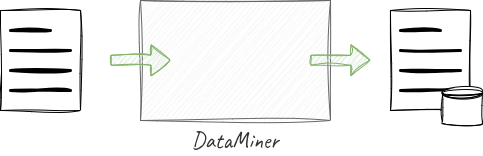
\includegraphics[scale=0.5]{./chapter/images/chapter_1.overview}
        \caption{Esquema general del sistema. \textit{Elaboración propia.}}
        \label{fig:chapter_1.overview}
    \end{center}
\end{figure}

\todo[inline]{@TODO: Mejorar la figura}

Tal y como se puede ver en la figura \ref{fig:chapter_1.overview}
el sistema recibe documentos y genera información en un formato estructurado.
El tipo de estructura, dependerá del tipo de documento.
Por ejemplo en un contrato de alquiler de vivienda aparecerán los datos de la vivienda, y en un contrato de compraventa
de vehículos, aparecerán los datos del vehículo.

    \chapter{Marco teórico}\label{ch:chapter_2}

\todo[inline]{@Marlene: colocas definiciones en las secciones pero no las referencias de esas definiciones
También debes relacionar cada seccion con tu trabajo Código limpio y arquitectura limpia pueden ir en una sola seccion
Si colocas una figura, debes referenciarla en el texto y explicarla}


\section{Código limpio}

\subsection{Introducción histórica}
El concepto de Código Limpio ha sido fundamental en la programación de software desde los primeros días del desarrollo
de software, pero fue articulado y popularizado con gran efecto por Robert C. Martin en su libro~\cite{book_martin_2008}

Este libro se convirtió en una guía esencial para muchos desarrolladores al enfatizar la importancia de escribir código
que no solo funcione, sino que también sea fácil de entender, modificar y mantener.

\subsection{Definición}
Código limpio es aquel que es fácil de entender y fácil de modificar.
Es elegante, eficiente y hace exactamente lo que se espera que haga.
Según Robert C. Martin, el código limpio puede ser leído y mejorado por un
desarrollador que no sea su autor original con un mínimo esfuerzo necesario.

Se caracteriza por su simplicidad, la ausencia de duplicación, la expresión clara de la intención del desarrollador, y
la atención a los detalles en el nivel de código.
Contiene los tests, no contiene errores y, lo más importante, revela claramente su diseño y propósito.


\section{Arquitectura limpia}

\subsection{Introducción histórica}
En el ámbito del desarrollo de software, la estructuración eficiente de la arquitectura de un sistema
es crucial para determinar su eficiencia, escalabilidad y mantenibilidad a largo plazo.

Una de las metodologías que ha cobrado relevancia en este contexto es la Arquitectura Limpia,
un enfoque sistemático para el diseño de software promovido por
Robert C. Martin.
En su libro Clean Architecture: A Craftsman\'
s Guide to Software Structure and Design (Martin, 2017), Martin presenta un marco de trabajo que prioriza la separación
de preocupaciones y la independencia de los diversos componentes del software.

\subsection{Definición}
La arquitectura limpia es un estilo de diseño de software que
organiza el sistema de manera que sea independiente de frameworks, UI, bases de datos y cualquier otra agencia externa.

\todo[inline]{@TODO: Insertar figura}
\todo[inline]{@Marlene: hay que referenciar en el texto la figura. Te falta colocar la referencia}

Representación de las comunicaciones entre capas en una arquitectura limpia.

La esencia de esta arquitectura radica en su diagrama concéntrico de capas, donde cada capa tiene responsabilidades
claramente definidas y depende solo de las capas más internas.
Esto se logra mediante el principio de Inversión de dependencias, lo que significa que los detalles dependen de las
abstracciones y no al contrario.

Aunque existen diferentes implementaciones de una arquitectura limpia, cada una con sus características intrínsecas, en
este proyecto hemos decidido implementar una versión en 3 capas.

\todo[inline]{@Marlene: mencionales. Aparecen 4 a continuación, por qué?}
\subsubsection*{Dominio}
Es el corazón del modelo de negocio de la aplicación y encapsula la
lógica y las reglas del negocio.

Esta capa es fundamentalmente agnóstica respecto a la aplicación de tecnologías externas y se
centra exclusivamente en cómo se comporta el negocio bajo diferentes condiciones y reglas.

Contiene entidades, objetos de valor, y dominios de servicio que representan y operan sobre los
conceptos fundamentales del negocio.

Esta capa debe ser autocontenida y fácilmente testable, aislada de influencias externas como bases de
datos o interfaces de usuario.

\subsubsection*{Aplicación}
La capa de aplicación actúa como un mediador entre la capa de presentación y la capa de dominio, coordinando
las operaciones de alto nivel que involucran múltiples aspectos del dominio.

\subsubsection*{Infraestructura}
La capa de infraestructura proporciona las capacidades tecnológicas necesarias para que las capas de
aplicación y dominio puedan realizar sus funciones sin tener que
preocuparse por los detalles de implementación de la plataforma o los elementos externos.

\subsubsection*{Presentación}
Es responsable de mostrar la información al usuario y de interpretar los
comandos del usuario para que la aplicación pueda entenderlos y actuar en consecuencia.

\todo[inline]{@Marlene: queda mejor si lo redactas como parrafo y no siguiendo ese estilo}


\section{Procesamiento de lenguaje natural}

\subsection{Introducción histórica}
El Procesamiento de Lenguaje Natural o Natural Language Processing (NLP) es un campo que se sitúa en la
intersección de la informática, la inteligencia artificial y la lingüística.

Se dedica al desarrollo de algoritmos y sistemas que permiten a las computadoras entender, interpretar y generar
lenguaje humano de una manera útil y significativa.
La historia del NLP comienza en la década de 1950, marcada por el trabajo pionero de Alan Turing y su famoso
test de Turing, que planteaba la cuestión de si una máquina puede emular el lenguaje humano de manera convincente
(Turing, 1950).

En los años 60 y 70, el enfoque inicial en la traducción automática
, como los esfuerzos del proyecto Georgetown, mostró tanto promesas como limitaciones significativas, lo que llevó a un
reajuste en las expectativas y métodos del campo (Hutchins, 2003).
Con la introducción de la inteligencia artificial (IA) en la década de 1980, surgieron métodos basados primero en reglas
y luego en modelos
estadísticos, culminando con el desarrollo de modelos de aprendizaje automático en la década de 1990 (Manning y Schütze,
1999).

El verdadero cambio paradigmático llegó con el advenimiento de las redes neuronales y el aprendizaje profundo
en la década de 2010.
Este período vio la creación de modelos de lenguaje avanzados, como BERT y GPT, que han revolucionado la capacidad de
las máquinas para procesar el lenguaje con un grado de sutileza y profundidad sin precedentes (Devlin et al., 2019;
Brown et al., 2020).

\subsection{Definición}
El NLP es un campo que combina técnicas de la informática, la inteligencia artificial y la lingüística computacional con
el objetivo de permitir que las máquinas entiendan, interpreten
, manipulen y generen lenguaje humano de manera efectiva y eficiente.

El NLP utiliza algoritmos y modelos matemáticos para abordar diversas tareas relacionadas con el lenguaje, tales como la
traducción automática entre idiomas, la generación de respuestas automáticas
, la extracción de información relevante de textos, el análisis de sentimientos, el reconocimiento de voz, y
la síntesis de habla, entre otros.


\section{Modelos de lenguaje de gran escala (LLMs)}

\subsection{Introducción histórica}
La historia de los LLMs comienza con los primeros modelos estadísticos de lenguaje en
la década de 1980, que utilizaban métodos simples como los modelos de Markov y n-gramas para predecir la probabilidad
de secuencias de palabras (Jelinek, 1997).
Estos métodos, aunque efectivos para algunas tareas básicas, estaban limitados por su incapacidad para capturar
contextos
más largos y por su dependencia de grandes corpus de texto para entrenamiento.

En la década de 2000, con el advenimiento de modelos más sofisticados como los modelos ocultos de Markov
y especialmente las redes neuronales, comenzó a vislumbrarse el
potencial de los modelos de lenguaje más complejos.
Sin embargo, no fue hasta la introducción de las redes neuronales recurrentes (RNN) y, más tarde, las redes neuronales
de memoria a largo plazo (LSTM)
que los investigadores pudieron abordar el problema del ''desvanecimiento del gradiente''
y mejorar significativamente la capacidad de los
modelos para aprender dependencias a largo plazo en el texto (Hochreiter Schmidhuber, 1997).

\subsubsection*{La revolución de los transformers}
El verdadero cambio paradigmático llegó en 2017 con el desarrollo de la arquitectura
Transformer por Vaswani et al.
Esta arquitectura introdujo el mecanismo de atención, que permite a los modelos ponderar diferentes partes de la entrada
de texto de manera dinámica, mejorando la capacidad de los modelos para manejar secuencias de texto largas y complejas (
Vaswani et al., 2017).

\todo[inline]{@Marlene: Transformers términos en inglés van en itálicas}

BERT, desarrollado por Google en 2018, y GPT, desarrollado por OpenAI, son ejemplos de
cómo los Transformers han sido adaptados para crear modelos que
no solo entienden el contexto de una palabra en función de su posición en una frase, sino en todo
el texto, permitiendo un entendimiento contextual mucho más rico (Devlin et al., 2019; Radford et al., 2018).

\subsection{Definición}
Los Modelos de Lenguaje de Gran Escala (LLMs) son sistemas
avanzados de inteligencia artificial diseñados para entender, generar y
manipular el lenguaje humano de manera coherente y contextualizada. Estos
modelos son entrenados en vastos conjuntos de datos textuales que abarcan una amplia variedad de temas, lo que les
permite desarrollar un conocimiento extenso sobre el lenguaje y sus usos prácticos.

Funcionan principalmente a través de técnicas de aprendizaje
profundo, especialmente usando arquitecturas como las de Transformers,
que permiten a los modelos captar relaciones complejas y contextos a largo plazo dentro de los textos. Este enfoque les
otorga la capacidad de generar respuestas, completar textos,
traducir entre idiomas, resumir información y responder preguntas con un alto grado de precisión y relevancia.

\subsection{Principales modelos}

\todo[inline]
{@Marlene: puedes hacer un resumen de estos modelos. Creo que no hace falta que coloques los código de ejemplos. Quizás
para un anexo}
\subsubsection*{OpenAI GPT}
ChatGPT es un avanzado modelo de lenguaje desarrollado por OpenAI,
basado en la arquitectura GPT (Generative Pre-trained Transformer).

Es uno de los modelos más reconocidos en la actualidad.
Aunque es un modelo privado, OpenAI ofrece acceso a través de una API de pago que incluye una capa gratuita limitada.

ChatGPT ofrece varios modelos, cada uno con un esquema de precios que varía según
su complejidad.
Una de las principales ventajas de este servicio es que proporciona una solución integral "plug-and-play", es decir, no
requiere instalación ni configuración adicional por parte del usuario.

A continuación un ejemplo de una llamada a esta API.


\subsubsection*{Hugging Face's Transformers}
Hugging Face's Transformers
es una biblioteca de procesamiento de lenguaje natural (NLP) que simplifica el uso de modelos de aprendizaje profundo
basados en la arquitectura Transformer.

Esta biblioteca ofrece una amplia variedad de modelos pre entrenados desarrollados por la comunidad
para fines específicos, además de la posibilidad de entrenar modelos personalizados.


Sin embargo, los modelos disponibles en Hugging Face suelen ser menos potentes que los modelos más
avanzados disponibles a través de plataformas como ChatGPT. ChatGPT ofrece
modelos con capacidades superiores, lo que puede ser una
consideración importante dependiendo de los requisitos específicos del proyecto.

\subsubsection*{Otros}
Además de OpenAI y Hugging Face, existen varias otras plataformas que ofrecen modelos de lenguaje
grande (LLM) para desarrolladores interesados en incorporar capacidades
avanzadas de procesamiento de lenguaje natural en sus aplicaciones. Entre
estas plataformas destacan Google AI, Facebook AI, NVIDIA NeMo y Microsoft AI, entre otras cada una con sus propios
enfoques y modelos distintivos.

%    \chapter{Capítulo tercero}\label{cap:cap3}


%% Anexos
%    \appendix
%    \chapter{Instrucciones adicionales}\label{ch:appendix_1}


El apéndice es toda la información adicional complementaria, necesaria para ilustrar mejor el cuerpo del trabajo.

Los apéndices van numerados con una secuencia alfabética de letras mayúsculas (A, B, C, etc.). En caso de que se hayan
producido diagramas de clases, diagramas de la base de datos, casos de usos u otra información gráfica y estos no hayan
sido incluidos como parte del cuerpo del trabajo, deberán ser incluidos en la sección de apéndices.

Apéndice A

Ejemplos formatos
El estilo del párrafo tiene que ser encuadrado (justificado).
En caso de terminar con un apartado (nivel uno de título) aplicar un salto de página para comenzar siempre el siguiente
apartado en una página nueva.

Tablas

Tanto las figuras como las tablas tienen que estar indicadas en el texto y referenciadas con la numeración que tiene
asignada.
La descripción debe ser clara y explicar lo que se quiere representar con independencia de la referencia del texto.

Tanto las tablas como las figuras tendrán un estilo de párrafo centrado.
La descripción se realizará desde “Insertar título”.


Tabla 1. Operaciones matemáticas utilizadas en el estudio realizado. Elaboración propia.

Figuras

Las figuras deben estar mencionadas en el texto y ser referenciadas por su numeración Ejemplo: Se habilita un servidor
con Jupyter como se puede ver en la Figura 1, en el cual se puede disponer de diferentes kernels de programación
(Python, R, Julia…).

Figura 1.
Arquitectura Jupyter Cliente - Servidor.
Fuente: https://www.paradigmadigital.com/dev/jupyter-data-science-aplicada/


Viñetado

Está permitido el uso de viñetado:

Esta sería la forma
Segundo
En caso de tener un sub apartado
Una numeración que se quiera hacer no debe influir en la numeración de los apartados generales:

1. Item 1
2. Item 2

%    \chapter{Instrucciones adicionales}\label{ch:appendix_1}


El apéndice es toda la información adicional complementaria, necesaria para ilustrar mejor el cuerpo del trabajo.

Los apéndices van numerados con una secuencia alfabética de letras mayúsculas (A, B, C, etc.). En caso de que se hayan
producido diagramas de clases, diagramas de la base de datos, casos de usos u otra información gráfica y estos no hayan
sido incluidos como parte del cuerpo del trabajo, deberán ser incluidos en la sección de apéndices.

Apéndice A

Ejemplos formatos
El estilo del párrafo tiene que ser encuadrado (justificado).
En caso de terminar con un apartado (nivel uno de título) aplicar un salto de página para comenzar siempre el siguiente
apartado en una página nueva.

Tablas

Tanto las figuras como las tablas tienen que estar indicadas en el texto y referenciadas con la numeración que tiene
asignada.
La descripción debe ser clara y explicar lo que se quiere representar con independencia de la referencia del texto.

Tanto las tablas como las figuras tendrán un estilo de párrafo centrado.
La descripción se realizará desde “Insertar título”.


Tabla 1. Operaciones matemáticas utilizadas en el estudio realizado. Elaboración propia.

Figuras

Las figuras deben estar mencionadas en el texto y ser referenciadas por su numeración Ejemplo: Se habilita un servidor
con Jupyter como se puede ver en la Figura 1, en el cual se puede disponer de diferentes kernels de programación
(Python, R, Julia…).

Figura 1.
Arquitectura Jupyter Cliente - Servidor.
Fuente: https://www.paradigmadigital.com/dev/jupyter-data-science-aplicada/


Viñetado

Está permitido el uso de viñetado:

Esta sería la forma
Segundo
En caso de tener un sub apartado
Una numeración que se quiera hacer no debe influir en la numeración de los apartados generales:

1. Item 1
2. Item 2


    \bibliographystyle{plain}
    \bibliography{./bibliography}

\end{document}
